% ============================================================
%  Poster template — Ciências ULisboa / Deep Learning class
%  Compile with: pdflatex poster_template.tex
%  Requires packages: geometry, tcolorbox, tikz, multicol,
%                     graphicx, fontenc, inputenc, lmodern
% ============================================================
\documentclass[a1paper, 14pt]{extarticle}
\usepackage[a1paper,
            left=1.2cm, right=1.2cm,
            top=0cm,    bottom=1cm]{geometry}

\usepackage[T1]{fontenc}
\usepackage[utf8]{inputenc}
\usepackage{lmodern}
\usepackage{graphicx}
\usepackage{xcolor}
\usepackage{tikz}
\usepackage{tcolorbox}
\usepackage{multicol}
\usepackage{enumitem}
\usepackage{booktabs}
\usepackage{array}
\usepackage{amsmath, amssymb}
\usepackage{url}
\usepackage{calc}

\tcbuselibrary{skins, breakable}

% ── Colours ─────────────────────────────────────────────────
\definecolor{ulblue}{HTML}{003A70}     % dark navy header
\definecolor{sectionbg}{HTML}{C8D8E8}  % light blue section header bg
\definecolor{sectionfg}{HTML}{003A70}  % section header text
\definecolor{bodytext}{HTML}{222222}
\definecolor{lightgray}{HTML}{F5F5F5}

% ── No paragraph indent, small skip ─────────────────────────
\setlength{\parindent}{0pt}
\setlength{\parskip}{4pt}

% ── Bullet style ─────────────────────────────────────────────
\setlist[itemize]{leftmargin=1.4em, itemsep=2pt, topsep=2pt}

% ── Section box style ────────────────────────────────────────
\tcbset{
  posterbox/.style={
    enhanced,
    colback=white,
    colframe=sectionbg,
    boxrule=2pt,
    arc=2pt,
    left=6pt, right=6pt, top=10pt, bottom=6pt,
    fontupper=\color{bodytext}\LARGE,
    attach boxed title to top left={yshift=-2pt, xshift=4pt},
    boxed title style={
      colback=sectionbg,
      colframe=sectionbg,
      arc=2pt,
      boxrule=0pt,
      left=4pt, right=4pt, top=3pt, bottom=3pt,
    },
    coltitle=sectionfg,
    fonttitle=\bfseries\normalsize,
  }
}

\pagestyle{empty}

% ============================================================
\begin{document}
% ============================================================

% ── HEADER ───────────────────────────────────────────────────
\begin{tikzpicture}[remember picture, overlay]
  \fill[ulblue] (current page.north west)
    rectangle ([yshift=-7.5cm] current page.north east);
\end{tikzpicture}

\begin{minipage}[t][4.2cm][t]{\textwidth}
\vspace{0.3cm}
  \color{white}
  \begin{minipage}[c]{0.18\textwidth}
    
\includegraphics[width=\linewidth]{ulisboa_logo.png}
    {\footnotesize Ciências ULisboa}
  \end{minipage}%
  \hfill
  \begin{minipage}[c]{0.60\textwidth}\centering
    {\Large\bfseries\itshape Semantically Supported Music Recommendations: Combining KG Representations of Musical Information with Heterogeneous Graph Transformers for Recommending New Music.}\\[10pt]
    {\normalsize\itshape Pedro Fanica$^{1}$, Aarthi Perumpillichira $^{2}$, Maja Skwaron$^{3}$}\\[5pt]
    {\small Student numbers: 54346, 66404, 66083}
  \end{minipage}%
  \hfill
  \begin{minipage}[c]{0.18\textwidth}\raggedleft
    {\small M.Sc.\ Data Science\\
    Deep Learning \& Knowledge Graphs 2025/2026}
  \end{minipage}
\end{minipage}

\vspace{2.5cm}

% ── MAIN BODY (two columns) ──────────────────────────────────
\begin{minipage}[c]{0.48\textwidth}

  % -- Objectives ----
  \begin{tcolorbox}[posterbox, title=Objectives]
    \begin{itemize}
    \item Build a music recommendation system that enriches standard collaborative filtering (CF) with musical features such as audio characteristics, genre, artist relationships, and instrumentation.
    \item Represent these features in a KG, capturing semantic relationships between users, tracks, artists, and genres that go beyond simple user-item interaction matrices.
    \item Train a Heterogeneous Graph Transformer (HGT) over this KG to learn richer representations, improving recommendation diversity, interpretability, and cold-start robustness.
    \end{itemize}
    \vspace{0.1cm} % placeholder space for optional figure
  \end{tcolorbox}

  \vspace{0.4cm}

  % -- Problem ----
  \begin{tcolorbox}[posterbox, title=Problem]
    \begin{itemize}
      \item Standard music recommendation collaborative filtering (CF) methods are based solely on user-item interaction history, ignoring the rich musical content of the songs themselves.
      \item Common approaches such as user-user CF or matrix factorisation suffer from popularity bias and cold-start failures for users or songs
      \item KG-enhanced methods address content sparsity by encoding musical relationships explicitly, but most prior work uses shallow KG embeddings without a GNN capable of propagating multi-hop relational structure.
      \item Can that gap be addressed by combining symbolic musical features with a heterogeneous KG and an HGT, enabling the model to reason over typed relationships such as shared genre, artist, or instrumentation?
    \end{itemize}
    \vspace{0.1cm} % placeholder space
  \end{tcolorbox}

  \vspace{0.4cm}

  % -- Methodology ----
  \begin{tcolorbox}[posterbox, title=Methodology]
    \begin{center}
      % Replace with your pipeline figure:
    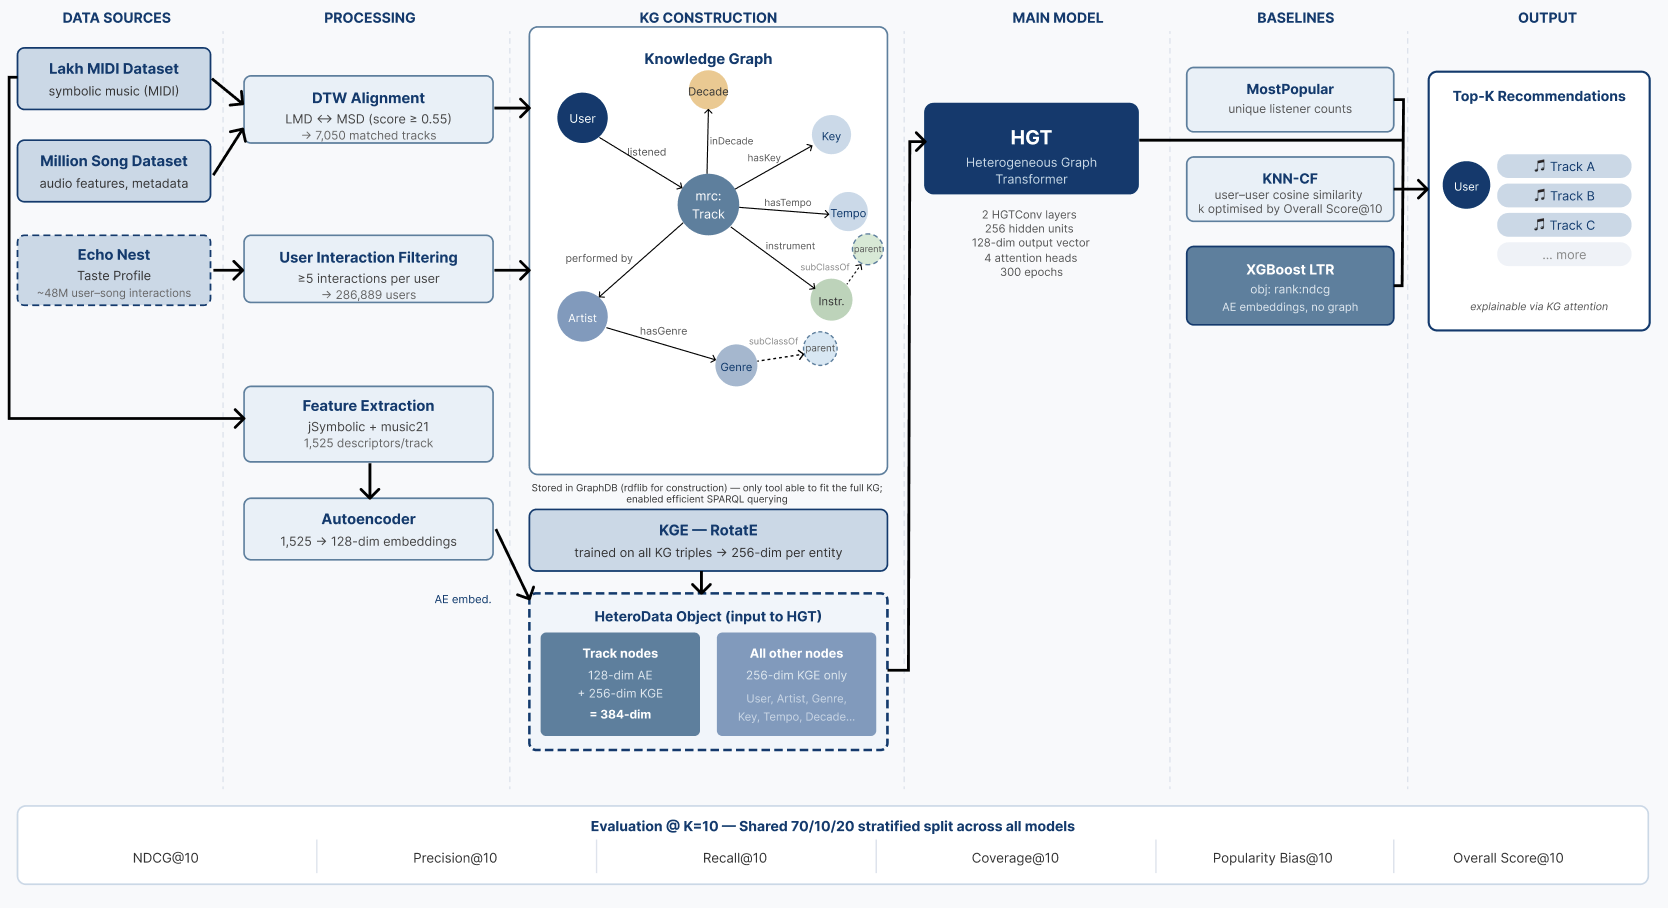
\includegraphics[width=0.97
    \linewidth]{pipeline.png}
    \end{center}
    \vspace{4pt}
    \begin{itemize}
    \item The composite \textbf{Overall Score} is defined as:
\begin{equation}
    \Large{\text{Overall Score@10} = 0.6 \cdot \text{NDCG@10} + 0.2 \cdot \text{Cov@10} + 0.2 \cdot (1 - \text{PB@10})}
\end{equation}
where Coverage rewards catalogue diversity and Popularity Bias is inverted so that lower bias yields a higher score. This formulation was chosen over a single ranking metric such as NDCG alone, as it jointly rewards relevance, catalogue diversity, and fairness, capturing the trade-offs inherent in a music recommender system where optimising purely for accuracy risks amplifying popularity bias and reducing coverage.
    \end{itemize}
  \end{tcolorbox}

\end{minipage}%
\hfill
\begin{minipage}[c]{0.48\textwidth}

  % -- Datasets ----
% \begin{tcolorbox}[posterbox, title=Datasets]
%   \begin{center}
%     \begin{minipage}[t]{0.48\linewidth}
%       \centering
%       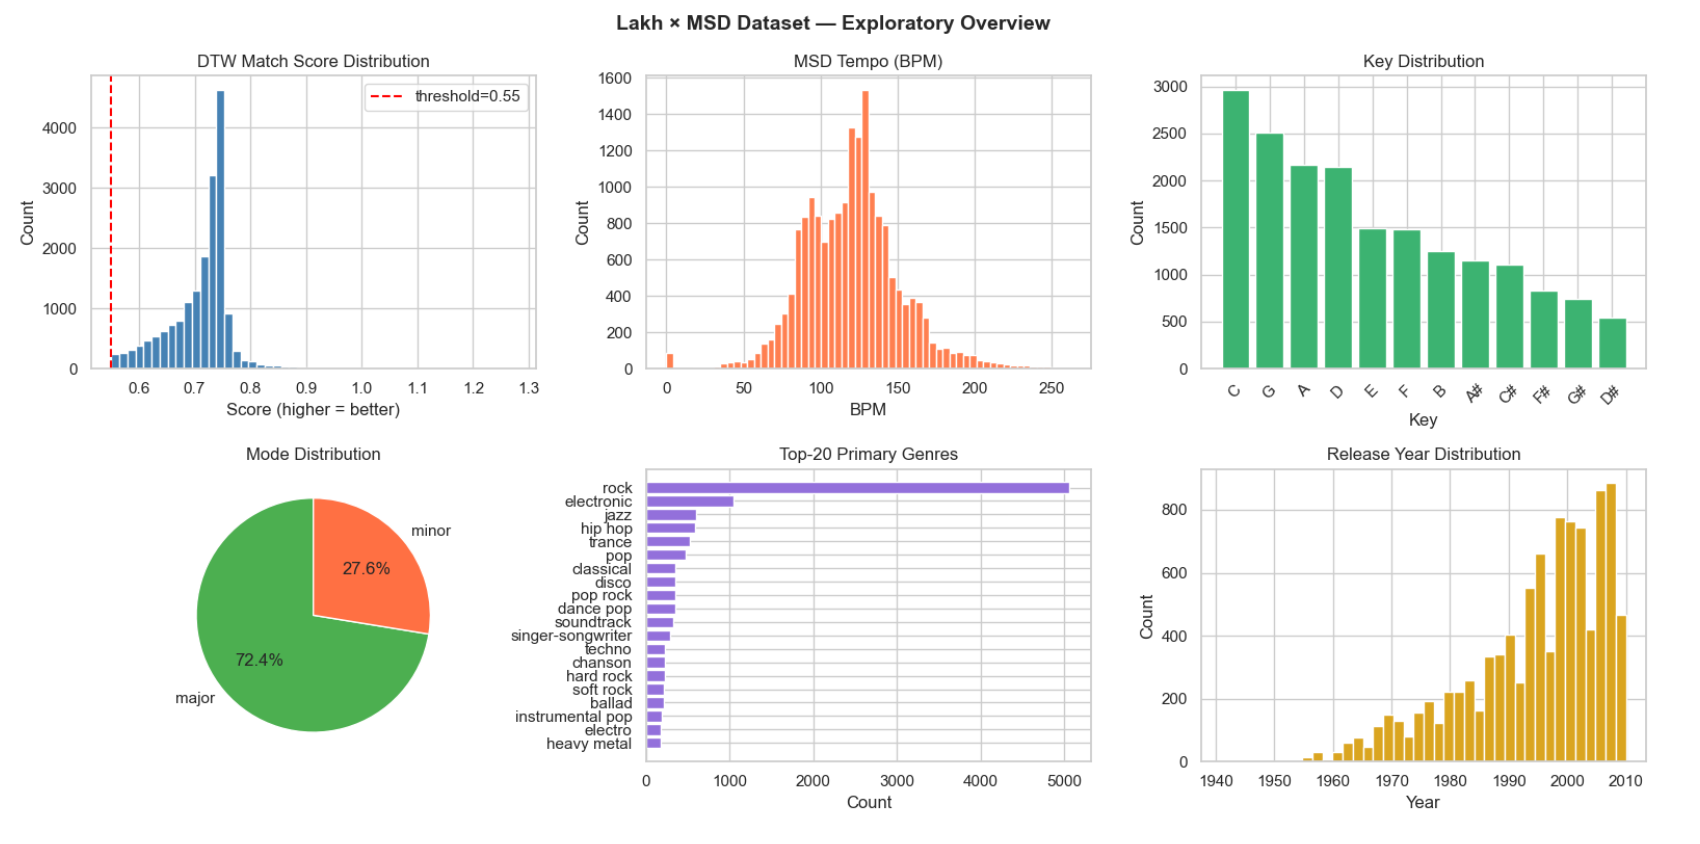
\includegraphics[width=\linewidth]{MSD_features.png}
%       {\small\textit{Exploratory overview of MSD feature distributions.}}
%     \end{minipage}
%     \hfill
%     \begin{minipage}[t]{0.48\linewidth}
%       \centering
%       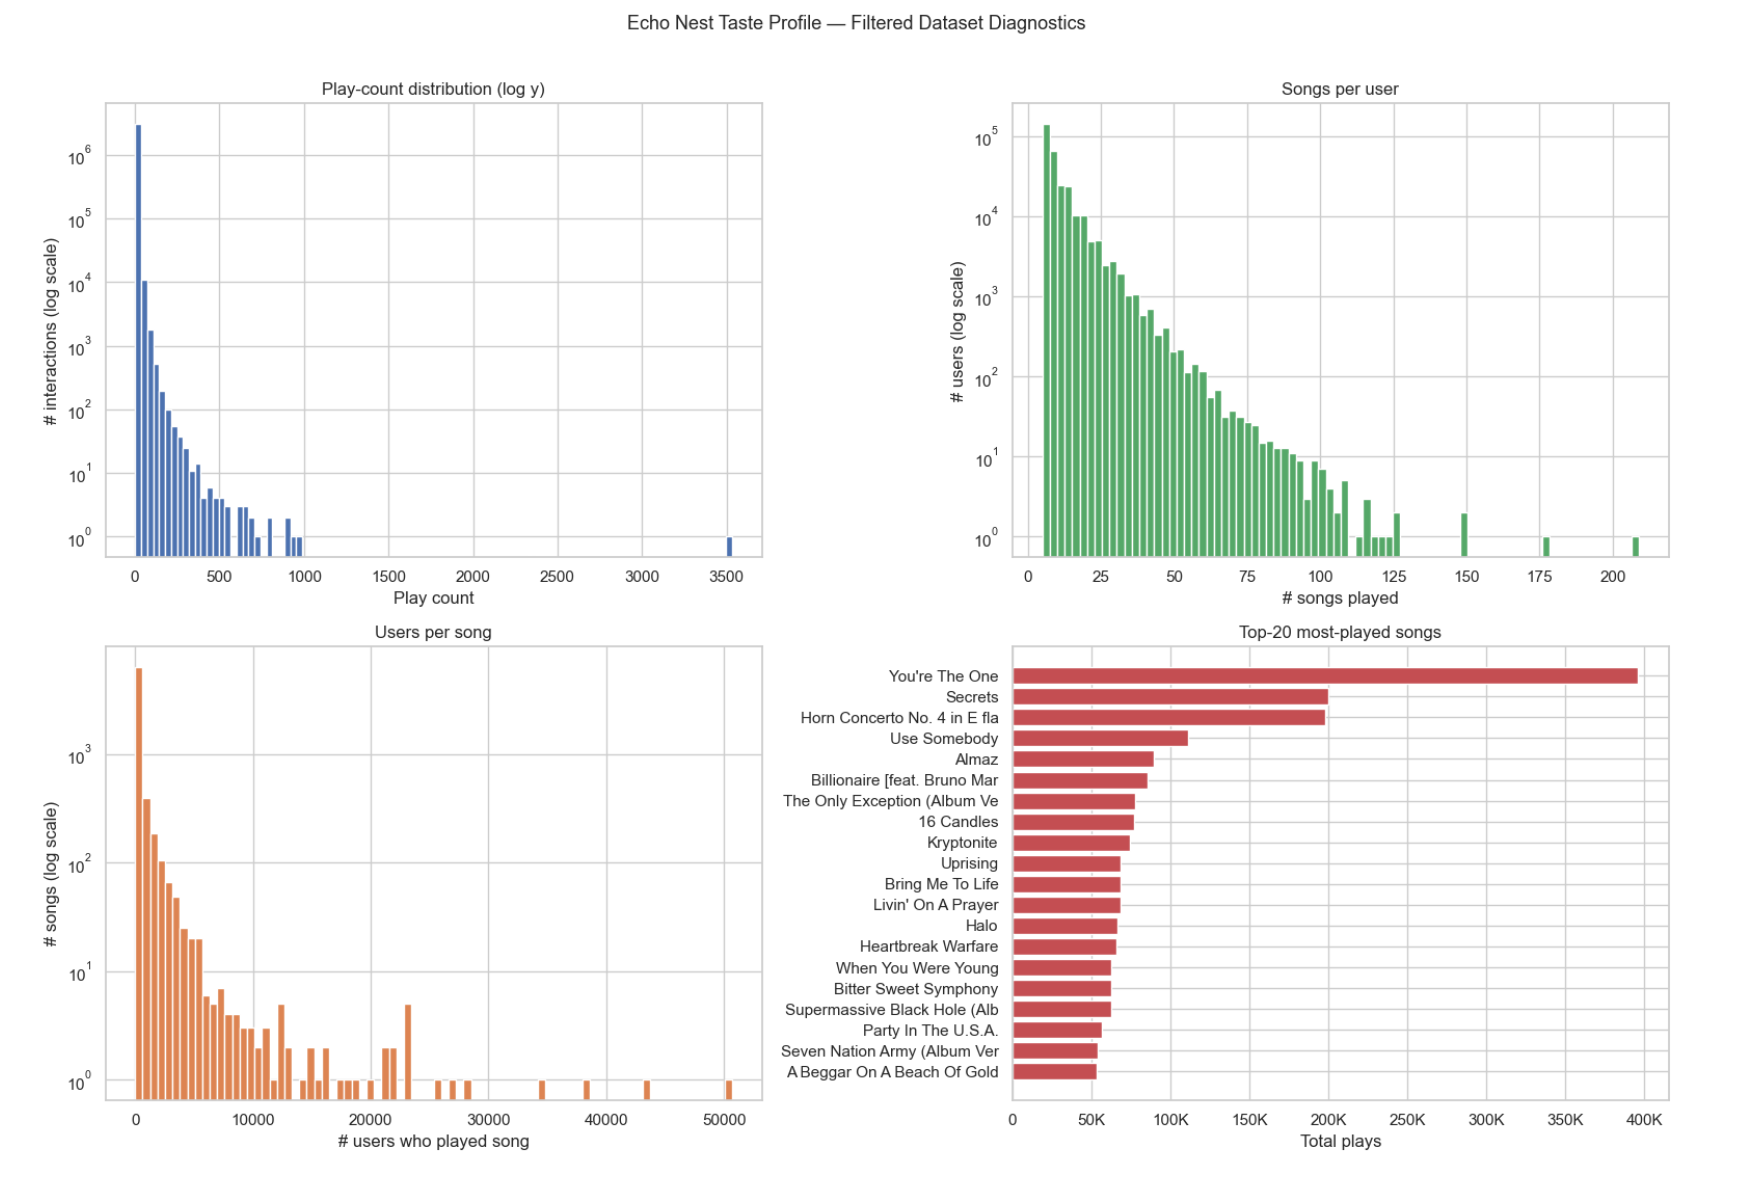
\includegraphics[width=\linewidth]{user_statistics.png}
%       {\small\textit{Play-count distribution, songs per user, users per song, and top-20 most-played tracks in the filtered Echo Nest Taste Profile.}}
%     \end{minipage}
%   \end{center}
%   \begin{itemize}
%     \item 286,889 users, 7,050 songs, aligned from Lakh MIDI + Million Song Dataset using DTW (threshold 0.55)
%     \item Songs described by both audio/metadata features (e.g. tempo, key, mode, genre, release year) and 1,525 numerical, symbolic music descriptors spanning seven categories: pitch, melodic, harmonic, rhythmic, dynamics, textural, and instrumentation.
%     \item User interactions from Echo Nest Taste Profile filtered to users with $\geq 5$ song interactions to address cold-start.
%     \end{itemize}
% \end{tcolorbox}

  % -- KG Results ----
  \begin{tcolorbox}[posterbox, title=KG Results]
  \vspace{6pt}
  \begin{center}
    % TBox — full width
    \begin{minipage}[t]{0.97\linewidth}
      \centering
      
\includegraphics[width=\linewidth]{TBox.png}
      {\small\textit{TBox of the MusicRecSys KG, showing ontology classes, properties, and Wikidata alignments}}
    \end{minipage}
    \vspace{8pt}
    \begin{itemize}
    \item The ontology is enriched via Wikidata entity linking: music genre instances are mapped to Wikidata classes via owl:equivalentClass (e.g. mrc:Genre $\longleftrightarrow$ wd:Q188451), while named individuals such as tempo markings (e.g. Allegro, Grave) and musical modes (Major, Minor) carry owl:sameAs links to their Wikidata counterparts. Decade individuals are chained temporally using Wikidata properties (e.g. wdt:P155/P156)(follows/followed by). 
    \item Blank nodes for \_:ListeningEvent and \_:GenreAssociation encode weighted, reified relationships (listen count per user-track pair; per-genre confidence weight per artist).
    \end{itemize}
    \vspace{3pt}
    % ABox + Table — side by side
    \begin{minipage}[t]{0.48\linewidth}
      \centering
      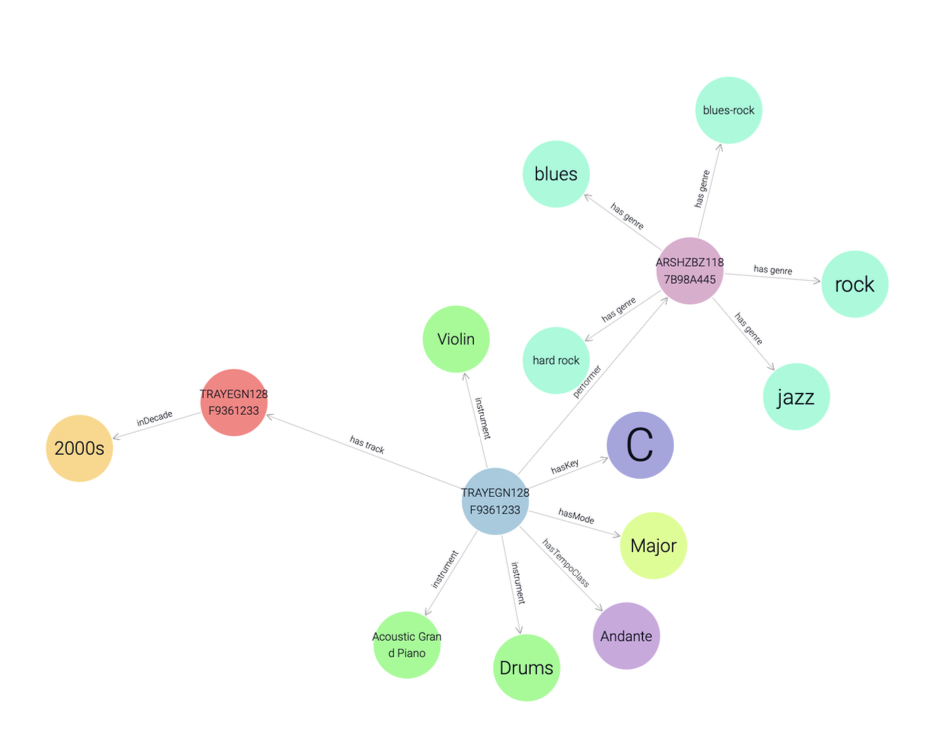
\includegraphics[width=\linewidth]{ABox.png}
      {\small\textit{ABox neighbourhood of track When She Dances as rendered in GraphDB.}}
    \end{minipage}
    \hfill
    \begin{minipage}[t]{0.48\linewidth}
      \centering
      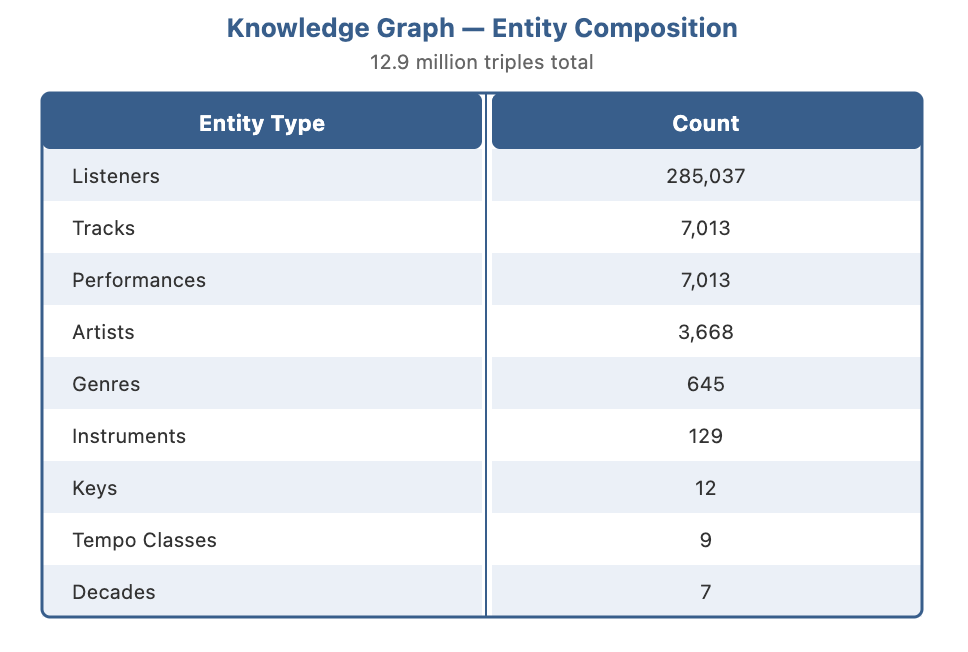
\includegraphics[width=\linewidth]{KG_summary.png}
      {\small\textit{Entity composition of the KG}}
    \end{minipage}
    \vspace{8pt}
    \begin{itemize}
        \item SPARQL genre ranking shows rock as the most frequent genre (2,117 artists), while average-weight ranking reveals that focused genres such as dance pop (0.81) and trance (0.795) rank above rock (0.759), reflecting that broadly tagged artists accumulate many low-weight associations, whereas niche artists tend to carry fewer but stronger genre tags. 
        \item High-confidence key queries (keyConf $\geq 0.8$) recover the expected Western-music prevalence of C (211 tracks), G (196), and D (150).
        \item The most listened tracks are: "Secrets" by OneRepublic (50,058 distinct listeners), and  "The One" by Dwight Yoakam (390,283 plays across 42,810 users).
    \end{itemize}
  \end{center}
\end{tcolorbox}


  \vspace{0.4cm}

  % -- Conclusions ----
  \begin{tcolorbox}[posterbox, title=Conclusions]
    \begin{itemize}
      \item Main takeaway
      \item Successes and failures
      \item Possible future directions
    \end{itemize}
  \end{tcolorbox}

\end{minipage}

\vspace{0.5cm}

% ── REFERENCES (full width) ──────────────────────────────────
% \begin{tcolorbox}[posterbox, title=References]
%   \begin{multicols}{3}
%   \footnotesize\setlength{\parskip}{1pt}\setlength{\columnsep}{10pt}
%   \noindent[1] Z. Hu et al. Heterogeneous graph transformer. \textit{WWW}, 2020.

%   \noindent[2] C. Raffel. Learning-Based Methods for Comparing Sequences. PhD thesis, Columbia Univ., 2016.

%   \noindent[3] T. Bertin-Mahieux et al. The million song dataset. \textit{ISMIR}, 2011.

%   \noindent[4] Z. Sun et al. RotatE: KG embedding by relational rotation. \textit{ICLR}, 2019.

%   \noindent[5] T. Trouillon et al. Complex embeddings for simple link prediction. \textit{ICML}, 2016.

%   \noindent[6] S. Rendle et al. BPR: Bayesian personalized ranking. \textit{UAI}, 2009.

%   \noindent[7] X. He et al. Neural collaborative filtering. \textit{WWW}, 2017.

%   \noindent[8] C. McKay et al. jSymbolic 2.2. \textit{ISMIR}, 2018.

%   \noindent[9] M. Cuthbert et al. music21, 2026.

%   \noindent[10] H. Wang et al. KG convolutional networks for recommender systems. \textit{WWW}, 2019.

%   \noindent[11] X. Wang et al. KGAT: KG attention network for recommendation. \textit{KDD}, 2019.

%   \noindent[12] X. He et al. LightGCN. \textit{SIGIR}, 2020.

%   \noindent[13] X. Liu et al. Music recommendation via KG and multi-task learning. \textit{Sci. Reports}, 2024.

%   \noindent[14] The Echo Nest. Taste profile subset of the MSD, 2011.

%   \noindent[15] Y. Raimond et al. The music ontology. \textit{ISMIR}, 2007.
%   \end{multicols}
% \end{tcolorbox}

% ── FOOTER ───────────────────────────────────────────────────
\vspace{0.3cm}
\begin{minipage}[c]{0.6\textwidth}
  \footnotesize\color{gray}
  Acknowledgements: This poster session is kindly sponsored by:
\end{minipage}%
\hfill
\begin{minipage}[c]{0.35\textwidth}\raggedleft
  % Replace with sponsor logo:
  % \includegraphics[height=1cm]{nttdata_logo.png}
  \color{ulblue}\textbf{NTT DATA}
\end{minipage}

% ── thin footer rule ──────────────────────────────────────────

\begin{tikzpicture}
  \draw[ulblue, line width=3pt] (0,0) -- (\textwidth,0);
\end{tikzpicture}

\end{document}
